\section{Above & Below}

We now describe the tooling we've built \emph{above}
the Graffiti API that makes development even easier, and
the implementations we've built \emph{below} the API
that realize different trade-offs between efficiency and
robustness.

While we have made insights on both fronts that at
the least demonstrate \emph{feasibility},
there are, of course,
many unanswered questions and unexplored ideas.
Fortunately, by having a static API in the middle, work done above the API
is \emph{decoupled} from work done below.
It is possible to drop in a new, more efficient, or privacy-preserving implementation
without upheaving all the tools and applications that have been built on top.
% Additionally, as mentioned, it is possible for different implementations to coexist,
% allowing for a smooth transition to a strictly better solution, akin the move from \texttt{http} to \texttt{https},
% or the perpetual coexistence of solutions, each with their own strengths.
% allowing for a smooth transition o
% It is also possible below for different implementations to coexist,
% much like how on top it is possible for different development frameworks
% to coexist.
% Implementations that are more efficient, secure can be developed independently
% of the high level tools and moreover switching will be easy.

% both above and below there is future work to be done.
% Low and now code tools and graphical editors.
% Efficient protocols.
% However by building this API in the middle
% we have \emph{decoupled} these two endeavors and they can
% proceed in parallel without being dependent or interfering on each other.

\subsection{Above}

While the API has hidden a lot of complexity below,
like the need to write and deploy server code or the need to
consider the server infrastructure at all,
writing JavaScript or TypeScript code is still inaccessible
to many people.
We have made some initial steps towards reducing the
programming complexity by allowing for the \emph{reactive} and
\emph{declarative} programming of Graffiti applications
and by providing a growing library of drop-in components for common designs.
We also point to a future where Graffiti applications could be built
without any code at all.

\subsubsection{Internal Synchronization}

When a user likes a post or sends a message,
it is necessary, for the usability of the interface, for the user
to get instant feedback that their action completed
successfully, by seeing a like counter increment or seeing their message
appear in the chat.
While it is possible to manually update the relevant sections of the UI,
this is unnecessary work for the developer and
can become unwieldy with many interconnected components.

Instead, we built a library for internal synchronization\footnote{
  \url{https://sync.graffiti.garden/classes/GraffitiSynchronize.html}
} that wraps around the Graffiti API to make these updates automatic.
Whenever the library encounters a new or changed object, either because
the user created, modified, or deleted an object,
or because an object was received from \texttt{get}
or \texttt{discover}, that change is internally forwarded to an
appropriate listener.
These listeners can be set up manually with the new methods \texttt{synchronizeDiscover}
and \texttt{synchronizeGet} or automatically by our Vue Plugin, described next.

% a user makes or receives a change, that change is internally forwarded
% to an appropriate listener.
% This library frosm the building block of reactivity that we build on
% in Section

% , set up with a new method \texttt{synchronizeDiscover}.



% This makes changes instant, without having to go over the network
% and require little additonal work

% Suppose one of a user's friends changes their name. As soon as the user's
% application receives one notice of that change (using get or discover),
% then synchronizeDiscover listeners can be used to update all instance's of
% that friend's name in the user's application instantly, providing a consistent user experience.

\subsubsection{Vue Plugin}

Vue is a popular frontend framework that enables ``reactive'' programming where
changes to the underlying state are automatically reflected in the UI.
We built a plugin for Vue\footnote{
  \url{https://vue.graffiti.garden/variables/GraffitiPlugin.html}
}
that provides a variant of
\texttt{discover} that returns a reactive array of objects rather than
an asynchronous stream.
Local user actions update the array automatically, thanks to
\texttt{synchronizeDiscover}, while remote changes
can be polled either manually with \texttt{poll()} or automatically
with an \texttt{autopoll} setting.
All updates to the array automatically propagate to UI components.
The plugin similarly provides reactive variants of \texttt{get} and
\texttt{recoverOrphans}.

% the array automatically while the \texttt{poll}
% function can be called to fetch remote changes.
% Vue lets all of these changes propogate automatically to UI components.

% operation to be returned reactively.
% The plugin combines the traditional

% We built a plugin for the Vue frontend framework that
% builds upon the internal syncrhonization library.
% The plugin combines \texttt{discover} with \texttt{syncrhonizeDiscover}
% and keeps a reactive array of all the results returned by a discover stream
% in
% Local changes update live, while remote changes can be polled by calling
% \texttt{poll}.
% It is still possible for a user to manually manage other \texttt{session}s
% for multi-actor applications.

The plugin exposes this reactive functionality with both
``composable'' functions,
% \footnote{
%   \url{https://vuejs.org/guide/reusability/composables.html}
% }
like \texttt{useGraffitiDiscover}, which can be used
in a more traditional programming environment, as well as
``renderless components,''
% \footnote{
%   \url{https://vuejs.org/guide/components/slots#renderless-components}
% }
like \texttt{<GraffitiDiscover>},
which can be used declaratively within an HTML template.
Additionally, for convenience,
the plugin sets up a global Graffiti class instance, \texttt{\$graffiti},
as well as a global
\texttt{\$graffitiSession}.
The plugin maintains complete TypeScript support and
is a relatively light wrapper over our internal synchronization library,
and so support for other front-end frameworks, like React, will be
fairly easy to add in the future.

Below is the complete code for a micro social application built with
the Vue plugin.\footnote{
  Try it out at \url{https://graffiti.garden/}
}
Once the application loads, the user can see how many people ``waved''
and can log in to wave themselves.
As soon as they click the 👋 button, the wave count updates automatically and
(with appropriate CSS) the button displays an animated waving motion.
If they click the button again, the waving stops and the count decrements.
Waves from other users also change the count, live.

\begin{lstlisting}[language=html]
<GraffitiDiscover autopoll
    v-slot="{ objects: waves, isInitialPolling }"
    :channels="[ 'https://graffiti.garden' ]"
    :schema="{
        properties: {
            value: {
                required: ['activity'],
                properties: {
                    activity: { enum: ['Wave'] }
                }
            }
        }
    }"
>
    <template v-if="$graffitiSession.value">
        <button
            v-if="!waves.some(
                wave => wave.actor === $graffitiSession.value.actor
            )"
            @click="$graffiti.put({
                value: { activity: 'Wave' },
                channels: [ 'https://graffiti.garden' ]
            }, $graffitiSession.value)"
        >
            👋
        </button>
        <button v-else
            class="waving"
            @click="waves.filter(
                wave => wave.actor === $graffitiSession.value.actor
            ).map(wave => $graffiti.delete(wave, $graffitiSession.value))"
        >
            👋
        </button>
    </template>
    <button v-else @click="$graffiti.login()">
        Log In to Wave
    </button>

    <p v-if="isInitialPolling">Loading...</p>
    <p v-else>{{ waves.length }} people have waved from this page 👋!</p>
</GraffitiDiscover>
\end{lstlisting}

\subsubsection{Component Library}

We have started compiling a library of Vue components
for common social functionality\footnote{
    TODO: Link to components library
}
such as \texttt{<GraffitiLike>} and \texttt{<GraffitiProfile>}.
The components are designed to be fairly extensible.
For example, a ``Like'' button can be configured to be a
``Dislike'' button by changing its \texttt{activity} and
\texttt{text} attributes.
Of course, for sufficiently unique applications, it will be necessary to
write custom components.

\subsubsection{Future Work}

There is certainly potential for more low- or even no-code tools
to be developed on top of the Graffiti API. It is an open
question as to whether it is possible to build an intuitive and completely
no-code system for Graffiti, like a graphical editor, without limiting
its extensibility.

Additionally, in our own application development,
we found that inline AI tools like GitHub Copilot are already
capable of generating large portions of functional Graffiti code.
This is especially true when writing applications with the
Vue plugin --- perhaps because of the reduction in boilerplate
code and the declarative nature of the templates.
It is not hard to imagine a future where a developer asks
a large language model to ``make a messaging app''
or to ``add a bookmark button to posts in this application'' and
it simply works.
% CITE
% https://www.geoffreylitt.com/2023/03/25/llm-end-user-programming

Finally, users may gravitate towards using ``meta'' applications.
Users of these applications could easily change their functionality
by swapping out different plugins,
which could represent different feed sorting algorithms
(similar to \cite{threeleggedstool, bluesky}),
different moderation policies, different styles,
or different features.
Or portions of applications may become represented within social objects themselves.
MySpace, for example, let users style their own pages --- what if users could easily add
custom social functionality to their own
or their community's ``pages''?

\subsection{Below}

Now we come to the problem of actually \emph{implementing} the Graffiti API.
As mentioned, an implementation can consist of multiple coexisting communication
\emph{protocols}.
We outline several communication protocols and their implementations first,
and then how they can be used in tandem.
% in a single implementation.

% We focus on scalability and trust.

% Finally, when there are multiple competing protocols,
% some user interface must be provided to the end user to choose which protocol
% they would like to use to \texttt{put} their own data
% as shown in Figure.
% some small amount of input on which protocol they would
% use to host their own data, however this decision can be remembered.
% can be remembered after they first call \texttt{put}.
% to
% \texttt{discover} can aggregate the results of \texttt{discover} from multiple protocols.
% Finally, there is the small problem of decided which protocol to use
% when an actor first \texttt{put}s an object.
% A URL includes within it a scheme that specifies which protocol to use.
% When calling \texttt{discover}, it can pull results from multiple
% different implementations and aggregate the results.

% j
% related to the Solid project,
% however it.
% A user logs in once to an \emph{identity provider} which then allows them
% to log in to various services.

% However a Solid OIDC only allows for webIds not other sorts of identity.
% It also has usability challenges - a user is asked to type in a URL.
% Chapi is attempting to fix this.
% We recommend to authors in this space to try to fuse the benefits
% of these protocols.

% but currently has shortcomings listed in Section~\ref{protocols}.

% The goal of systems \emph{below} the API is to make sure the
% API is implemented efficiently, scalably, and to provide \emph{trust}.
% For example, we could implement

\subsubsection{Local Protocol}

Our first ``protocol'' is one that runs locally
and handles objects with the URL scheme \texttt{graffiti:local:}.
Any data created on the local protocol is only visible on the device
it was created on.
While such a restriction may seem like a non-starter for an implemetation
of our \emph{social} API, it is invaluable for development.
It provides a similar functionality to running a \texttt{localhost} development server,
however it runs within the implementation of the API itself and so
does not require the complexity of standing up a local server.
Developers can easily create test actors and test objects on the local protocol
without polluting their own online presence or existing Graffiti applications.
% Our implementation of this protocol also includes its own internal
% identity provider allowing for the creation of various test actors.
Finally, the protocol is accessible in deployed applications
and lets regular users try a Graffiti application out without
having to create or log in to an account, as shown in
Figure~\ref{above-and-below:login}.

\begin{figure}
    \label{above-and-below:login}
    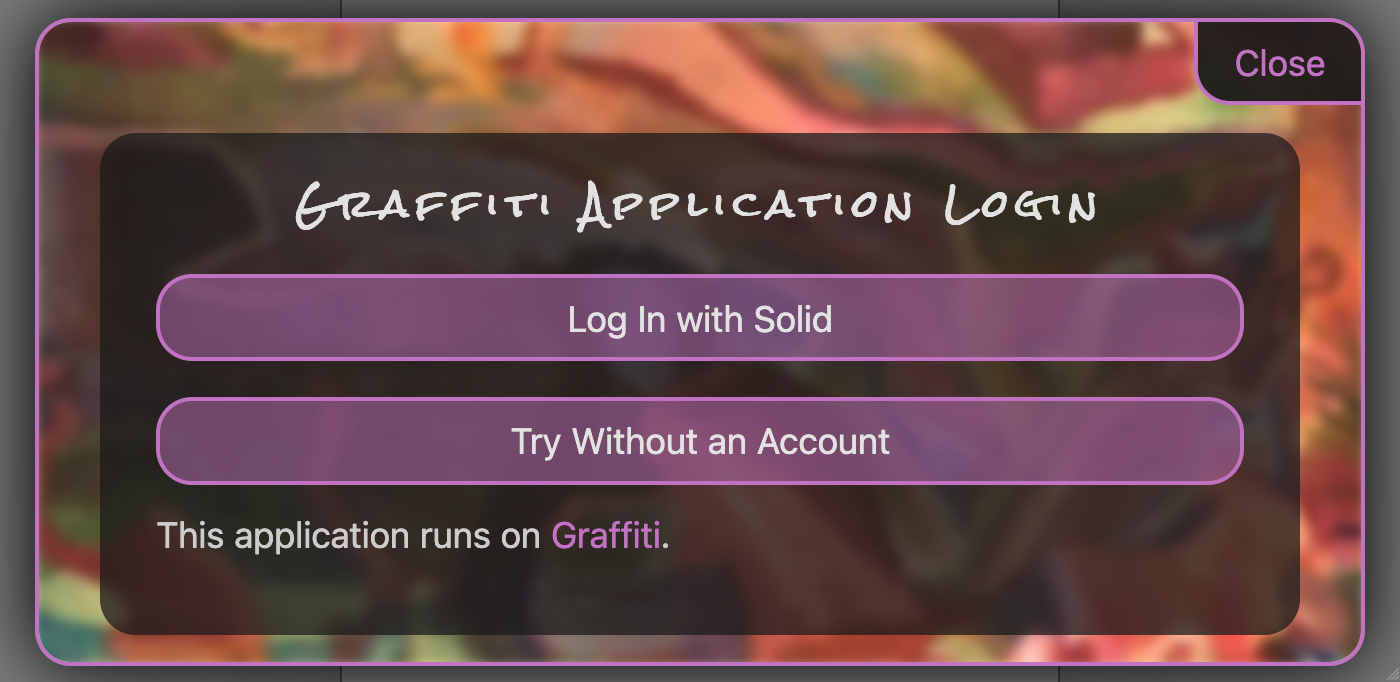
\includegraphics{figures/login.png}
    \caption{The modal that pops up when the user triggers a \texttt{login()}. TODO: Update the figure to show the whole flow.}
\end{figure}

We implemented the local protocol\footnote{
    \url{https://github.com/graffiti-garden/implementation-local}
} using PouchDB, a Javascript library that allows for persistent
storage in both the browser and in node.js.
Because of its relative simplicity, the local implementation also serves
as a reference implementation of the Graffiti API and pieces of its code are also used
throughout other implementations.

% Since Graffiti implementations can coexist by using different URL schemes,
% it is possible to use the local implementation in tandem with other implementations.
% This lets a user try out Graffiti applications without having to create an
% account. The data they use in the trial will simply only be visible locally but
% not available to others. At this time the data cannot be transferred once
% a user decides to create an account, but this is scheduled to be added in the future.

% Our local implementation builds on PouchDB which provides persistent
% storage both in the browser and in node.js.
% and pieces of its implementation are used in all of the other implementations.

% The local implementation is an implementation of Graffiti where all data is stored
% locally and only availble on one device. While this seems strange for a tool
% proported to build social applications, it is paramount to the developement experience.
% It allows for rapid iteration and testing, and creation of users.

% When a user calls "login()" in the local implementation, a popup appears that
% simply asks them to type in their actor ID, no additional authentication is required.
% They don't need to worry about polluting their own online presence with test data.
% Once an application it can be swapped out seamlessly with any of the other applications
% by just changing one line of code.

% Our local implementation builds on PouchDB which provides persistent
% storage both in the browser and in node.js.

% A local implementation is possible to be used

% Additionally, it also makes it possible to have hybrid implementations,
% that draw from multiple sources.

\subsubsection{Remote Protocol}

The remote protocol maps the Graffiti API onto
a monolithic HTTP server.
The protocol is a relatively straightforward transformation of
Graffiti's API methods to HTTP requests: the CRUD operations
easily translate to HTTP PUT, GET, PATCH, and DELETE while
\texttt{discover}, \texttt{recoverOrphans}, and \texttt{channelStats}
are additional POST endpoints.
Object URLs start with the scheme \texttt{graffiti:remote:}
followed by the domain name of the server and the
path to the object. The result is similar to a traditional
web URL only with \texttt{https://} replaced by \texttt{graffiti:remote:}.
For example, \texttt{graffiti:remote:pod.graffiti.garden/123}.

When there is only one server in use, the protocol is essentially
\emph{centralized} which is extremely efficient and scalable but requires
enourmous trust in the central server.
Alternatively, with multiple servers deployed,
a user can choose which they would like to use to store their own data
(see Figure~\ref{above-and-below:choose-protocol})
and their client can call \texttt{discover} on
multiple servers and aggregate the results,
allowing the user to communicate with others regardless
of their choice of server.

This network topology is an example of \emph{federation},
a form of decentralization, which is used by most of the
existing social protocols that we survey in Section~\ref{related-work},
as well as familiar services like email.
Federation provides defense against a centralized entity
co-opting the network.
However, our use of it here begs the questions:
How does a client know which servers to federate with?
How can an actor authenticate with multiple servers?
We answer these questions and others below.

% There are several questions:
% \begin{enumerate}
%     \item How does a client application know which servers to query?
%     \item How can actor authenticate with multiple servers to receive
%     private objects?
%     \item How can a client application verify that an object
%     was created by a particular actor?
% \end{enumerate}

\paragraph{Server Discovery}

The simplest way for a client to know which
servers to query is for there to
be a public ``registry'' of servers.
This is the method used by BlueSky~\cite{bluesky}
% and by other federated services like
% the \texttt{apt} package manager
% certificate authorities
% and package managers
and is available in our
own implementation.
A registry is simple, but it is a potential central point of control
and it does not allow for new
servers to easily enter the network.
Additionally, if there are too many servers, a registry can become
incredibly inefficient as each \texttt{discover} operation needs to be called
on \emph{every} registered server, when it is likely that relavent data
will only exist on a sparse subset of servers.

We provide a more decentralized and efficient
solution that works \emph{on top} of the remote protocol,
however it is involved enough that we consider it its own sub-protocol.
We discuss it in Section~\ref{above-and-below:announce-protocol} after introducing the concept
of a \emph{tracker}
in Section~\ref{above-and-below:commodity-storage-protocol}.

\paragraph{Authentication}
Actors in the remote protocol are authenticated with an existing
identity protocol called Solid OIDC.
Solid OIDC allows an actor to log in \emph{once} to an
``identity provider'' (see Figure~\ref{above-and-below:login})
and then silently authenticate with multiple
other servers.
The user's actor URI is a URL called a \emph{webId}.
We discuss Solid OIDC and identity in general in our discussion of
coexisting protocols, Section~\ref{above-and-below:coexisting-protocols}.
% with different
% which provides a webId.
% We will delve into identity later when we talk about coexisting protocols
% Our implementation of the remote protocol builds upon
% our implementation of the local protocol.

\paragraph{Delegation}
\label{above-and-below:delegation}

When a remote server returns an object that it claims
was created by a particular actor, how can the client verify that claim?
Many decentralized systems use public key cryptography to sign messages,
however this has the potential to disable \emph{repudiation},
violating requirement~\ref{requirements:forgiving}.

Instead, we use delegation. When a user first \texttt{put}s an object
to a new remote server, they mark that server as ``delegated'' in their
webId \emph{document}. This document is public and so others can verify
that the user has delegated permission to the server.
Once an actor deletes an object from a server there is no
``paper trail'' still connecting them to the object.

The webId document can also be used to set up "forwarding rules" for
situations where an actor wants to move their data from one server to
another without breaking all their object's \texttt{url}s.
This enables \emph{data portability}.

% As we saw in \cref{identity-provider}, the Solid OIDC specification
% allows a user to store some amount of data at their webId.
% That data is a URL which points to a Graffiti object owned by the user
% on some pod, and includes global settings.
% These settings include a list of

% The settings also include forwarding rules which allow a user to

% The verification of these settings is done by the client core library.

% The issue of the federated implementation is delegation.
% Which pods does a user say they want to do?
% It becomes necessary for the Actor to link to a "settings" document
% containing delegation and forwarding rules.
% This means there are no signatures which would violate the deniability property.

\paragraph{Implementation}

Our implementation of the remote protocol server\footnote{
    \url{https://github.com/graffiti-garden/implementation-remote}
} wraps our local implementation behind
a web server built on node.js with NestJS and Fastify.
We point the local implementation's PouchDB instance
to use a CouchDB database for efficiency and robustness.
We also use a library from the Community Solid Server project
for Solid OIDC authentication~\cite{communitysolidserver}.
The server is bundled as a Docker image for easy
cross-platform deployment.

The client-side library makes sure to validate
incoming data and to verify delegation in case a server attempts
to lie or otherwise misbehave.

\subsubsection{Commodity Storage Protocol}
\label{above-and-below:commodity-storage-protocol}

An alternative Graffiti protocol builds on top of existing
\emph{commodity storage} providers,
similar to Dropbox.
While the protocol is less efficient than the remote
protocol, its bootstrapping off of existing
storage solutions makes it more familiar and robust.
A user does not need to worry that an experimental new service
will go offline or lose their data.
% Additionally, storage providers have already established
% a viable economic model with a freemium tier and paid service
% for more storage or bandwidth.
% A user does not need to worry about an experimental new service going down.
% However they post performance issues:

At a high level, the protocol works as follows.
Actors on the protocol store their objects on a storage
provider of their choice.
Their client manages channel-specific files on that provider,
each containing all the objects the actor has published to that channel.
A user's client shares links to those channel files
with a \emph{tracker}.
The tracker is similar to a BitTorrent tracker~\cite{bittorrent} but
rather than mapping torrent IDs to IP addresses
it maps channel strings to channel file URLs.
To run \texttt{discover}, a client queries the tracker
about each channel of interest,
and then fetches each of the resulting URLs for objects.

% More specifically, to \texttt{put} a new object, a client
% performs the following:

% \begin{enumerate}
% \item
% If this is the first time the storage service is being used
% for Graffiti,
% create a directory called \texttt{graffiti} and
% within it directories called \texttt{objects} and
% \texttt{channels}.
% \item
% Create a file containing the object's
% \texttt{value} and \texttt{actor} and store it in the
% \texttt{objects} directory with access control
% set so that only actors in the object's \texttt{allowed} list
% can access it.
% \item
% Create a sharable link to this object
% to use as its \texttt{url}.
% \item
% For each of the object's channels, create a file for it
% within the \texttt{channels} directory, if it does not
% already exist, like \texttt{channels/my-channel}.
% Then add the object's \texttt{url} to the end of the file.
% \item
% Create a sharable link to each channel-specific file
% and publish it to the tracker, if not already done.
% \end{enumerate}

There is some additional bookkeeping that must be done to
keep objects in multiple channels in sync, and to enforce an object's
\texttt{allowed} list using the storage provider's built-in access control,
but we've omitted those details for brevity.
% The procedure of \texttt{discover}ing an object happens essentially in
% reverse.
% Some additional bookkeeping and privacy details have been ommitted for brevity.
Additionally, like the remote protocol, the commodity storage protocol
relies on delegation for verifying that an object was created by a particular actor.

The commodity storage protocol is less efficient than the remote protocol because each
\texttt{discover} call requires a network request per-channel-per-actor,
where as the remote protocol requires only one request per remote server.
If, like email or Mastodon, many actors, especially those in regular contact
use the same server~\cite{mastodonchallenges},
then \texttt{discover} on the remote protocol can take as
few as \emph{one} request while requests made by
the commodity storage protocol scale with the number of actors.
Additionally, the schema provided to \texttt{discover} cannot be used for any
server-side filtering --- a client must download \emph{all} objects in a channel
and discard ones that do not match the schema.
Still, for users who tend to participate in small networks, these issues
of scale are not a concern and the use of ``simple'' storage servers can be appealing.

We implemented the commodity storage protocol
% \footnote{
%     TODO link to solid implementation
% }
on top of a custom tracker\footnote{
    \url{https://github.com/graffiti-garden/link-service},
    \url{https://github.com/graffiti-garden/link-service-client}.
    WebTorrent was considered instead of a custom tracker,
    but unfortunately it does not persist announcements more than a few hours.
} and the Solid protocol.
For our purposes, Solid is essentially a federated form of Dropbox.
% where people can stand up their own Dropbox instance.
It also shares the same identity system as our remote protocol,
which we discuss in Section~\ref{above-and-below:coexisting-protocols}.
Objects stored on the protocol have URLs that start with \texttt{graffiti:solid:}.

\subsubsection{Announce Protocol}
\label{above-and-below:announce-protocol}

To resolve the issue of server discovery in the remote protocol,
a tracker-like service can be built on the protocol itself.
When an actor publishes an object to a small, perhaps self-hosted
server their client also publishes an \texttt{"announce-server"}
activity, pointing to their small server, on several ``well-known'' servers.
To handle an actor's \texttt{discover} request, a client first \texttt{discover}s
for \texttt{"announce-server"} activities on each of the well-known
servers and then makes the original \texttt{discover} request on each
announced server.
Announce activities are only posted to the channels
that an actor has published to, ensuring that a client
will not unnecessarily call \texttt{discover} on servers
that have no objects.

This protocol is guaranteed not to miss objects so long as
the posting actor's ``well known'' servers overlap with the
\texttt{discover}ing actor's.
We are assuming again that, like email or Mastodon, there are several
``large'' servers, like Gmail or mastodon.social, that can be used as these
rendezvous points.

By implementing the tracker using Graffiti objects,
it is possible to flexibly add new features to the tracker
in the same way that it is possible to flexibly add
functionality to any other Graffiti object.

We developed a proof of concept implementation of the announce protocol\footnote{
    \url{https://github.com/graffiti-garden/implementation-federated}
},
however it is not currently in use as the Graffiti ecosystem is not
large enough for it to be relevant.
It is not possible for the commodity-storage protocol to implement
the announce protocol, removing the need for a tracker,
because commodity storage servers do not allow clients to
query multiple users' data at once.

\subsubsection{Coexisting Protocols}
\label{above-and-below:coexisting-protocols}

The Graffiti API is designed so that different underlying
communication protocols can be used together with relative ease.
An object's URL starts with a scheme that indicates
how the various CRUD methods should resolve and interact with the object.
For \texttt{discover}, multiple protocol-specific \texttt{discover} calls can be
aggregated into one stream.

The first time a user attempts to \texttt{put} an object,
they must indicate which protocol they would like to use
as well as other protocol-specific information, such as what
remote server they would like to use.
To avoid confusing users we have tried to make this experience
as frictionless as possible, with reasonable defaults for
users who do not care about the underlying infrastructure,
as shown in Figure~\ref{above-and-below:choose-protocol}.
As mentioned in Section~\ref{above-and-below:delegation},
a user can later migrate their data to a different protocol
or server without breaking their object's URLs.

\begin{figure}
    \label{above-and-below:choose-protocol}
    TODO: this will be a figure!!
    \begin{itemize}
    \item
    Panel 1: Where would you like to store your data? You can always change this later.
    "Choose for Me", "On a Graffiti Server", "On a Solid Pod".
    \item
    Panel 2 (Graffiti): Which Graffiti server would you like to use?
    \item
    Panel 3 (Solid): Which Solid pod would you like to use?
    \end{itemize}
    \caption{The modal that pops up when the user triggers a \texttt{put()} for the first time.}
\end{figure}

For two protocols to truly coexist,
\emph{identity} must also be portable across them.
For example, it should be possible for an actor who stores their data on
the commodity storage protocol to send a private message to an
actor who stores their data on the remote protocol.
Currently, this is indeed possible, because both protocols use Solid OIDC
and the local protocol uses a compatible internal ``identity provider.''

Unfortunately, Solid OIDC is incompatible with many familiar
identity solutions, like ``Log in with Google,''
and many novel identity solutions, like ``Sign in with Ethereum.''
The Decentralized Identifier (DID) specification attempts to unify
these various identity methods, but currently DIDs require that
users log in with \emph{each} service they want to authenticate with~\cite{dids}.
This is like requiring a user to log in again every time
they receive an email from a new email server, which would
be tedious and confusing.
We hope that DIDs or new specifications evolve past this restriction.

% Solid OIDC has some shortcomings
% In the future we would like to support a more extensible identity system
% Solid OIDC is useful for us because it allows a user to log in once.
% However it makes some strong assumptions about identity on the web and
% has left over baggage from the Solid's semantic web vision that can be confusing to users.
% A more recent and extensible Decentralized Identifier is more extensible
% --- identity can be stored by various ``methods'' like \textttt{did:eth:}
% for storing an identity on ethereum.


% such a universal identity standard does not yet exist
% and developing one is outside the scope of this paper.

% The Decentralized Identifier (DID) specification~\cite{dids}
% is an attempt to unify various identity systems, decentralized and centralized.
% % is \emph{almost} sufficient.
% A DID is a URL and, like web URL or a Graffiti object URL,
% the scheme at the beginning of the URL indicates how it should be
% \emph{resolved}.
% For example, a DID with the scheme \texttt{did:web:}
% can be resolved by fetching a web document, where as
% a DID with the scheme \texttt{did:eth:} can be resolved by querying
% the Ethereum blockchain.
% A DID resolves to a \emph{document} that specifies \emph{methods}
% to authenticate the DID.

% Unfortunately, DID authentication methods prove the user's identity
% to only \emph{one} service.
% In the case of Graffiti, this means that a user would have to log in
% once for each underlying server they want to receive private data from,
% which is repetitive for the user and exposes them
% to the complexity of the underlying infrastructure.
% Instead, we would like the the user to be able to only log in \emph{once} to establish a \texttt{session}
% which can then be reused for all interactions.

% Therefore, we are using an earlier identity solution called Solid OIDC.
% Solid OIDC is less extensible, carries over some unneeded baggage from the Solid project,
% and has some usability issues.\footnote{
%     URLs are unnecessarily long.
%     The Solid OIDC specification also provides
%     each user with a webId, a globally unique and human-readable URL
%     that can be shared like a username or an email address.
%     At this URL, the user can store a small amount of public data
%     which we use to implement "delegation".

%     Additionally, existing OIDC servers generate their own
%     webIds, which are often verbose,
%     \emph{e.g.} \url{janedoe.solidcommunity.net/profile/card#me}.
%     There is no reason why a user could not come with their own, simple, domain name, for example
%     \url{id.janedoe.com}, similar to the AT Protocol~\cite{bluesky}. This would also give the users the ability
%     to switch identity providers while maintaining their identity.
%     It is not also currently easy to generate throwaway webIds
%     which could be useful for one-time or anonymous interactions.
% }
% However, a user only logs in \emph{once} to an ``identity provider'' which then
% silently authenticates the user with various services.
% It can also be decentralized, allowing the user to change providers.

% We have implemented this specifically on top of Solid.
% Object URLs start with \texttt{graffiti:solid:}
% This is because it has portable identity,
% where as Dropbox requires each application to register an API key
% and locks in to a partciular mode.
% - Dropbox does not provide a portable identity and becomes a centralized point of control.
% It is also not possible for access control to happen between platforms like Dropbox and Google Drive.
% This is not a problem for Solid, but Solid is unfamiliar and not as robust.
% - With Dropbox application developers need to register an application key.
% We use Solid as our storage provider because it provides
% a more open API and a portable identity system.
% We discuss identity in more detail in section X.

% Using a commercial storage provider like Dropbox allows for access control but only if users
% have a Dropbox account, which locks users into a proprietary service.
% Solid does not have this problem. In fact, it is not possible to use the Dropbox API
% without being used into a Dropbox account, but it is possible to use the Solid API
% without being locked into a Solid account.

\subsubsection{Future Work}

The remote protocol offloads work to complex storage servers,
while the commodity storage protocol shifts work to clients, keeping the servers simple.
A middle ground could be created where slightly more information is given to
the \emph{tracker}, like when a channel was last modified
or some schema-based indexing of channel content,
to allow for more efficient \texttt{discover} calls.

In the commodify storage protocol, the tracker also serves as a central point of control and so, like in BitTorrent,
it could be replaced with a distributed hash table~\cite{bittorrentdht}. In small networks,
a tracker may not be necessary at all and can be replaced with a gossip protocol.

Currently each server owner can see all the objects and channels
that pass through it. While federation allows users to switch
to servers they trust, those servers are still vulnerable to
subpoenas, putting groups like activists at risk.
It would be valuable to build end-to-end encrypted versions of the remote servers,
tracker, and commodity storage servers, perhaps building on
searchable encryption~\cite{searchableencryption}.

% Finally, non-federated architectures like a peer-to-peer
% implementaiton may also be possible.
% To our knowledge it is not directly possible to implemenet
% Graffiti on top of ecosystems like the AtProtocol or ActivityPub
% without leaking channels. However encrypting data may
% work.

% service where a lot of the work is done on individual
% servers and the commodity storage protocol demonstrates one where.
% There are indexes.
% There are also ways of fusing ideas from both the
% commodity storage and
% The remote implementation maps
% tracker: channel->objects
% It requires all servers in the system to be relatively complex.
% The tracker implementation maps
% tracker: channl->directories
% Most of the servers are \emph{simple}
% but the system is inefficient.
% There is a middle ground where slightly more information
% is given to the tracker, but

% There is much more work to be done making.
% For example, in cases like private messaging where a user
% is continually polling for an object a protocol should silently
% ``upgrade'' to a bidirectional socker.
